\documentclass[a4paper]{article}

\usepackage[english]{babel}
\usepackage[utf8]{inputenc}
\usepackage{amsmath}
\usepackage{graphicx}
\usepackage{hyperref}
\usepackage[colorinlistoftodos]{todonotes}
\usepackage{float}
\usepackage{geometry}

\title{STLDD - Software Top Level Design Document}
\author{Team 2}

\begin{document}
\begin{titlepage}
\newgeometry{left=2cm,top=1cm,right=2cm}
\newcommand{\HRule}{\rule{\linewidth}{0.5mm}}

\begin{minipage}{0.5\textwidth}
\begin{flushleft} % Responsible persons, write on separate lines
\textit{Responsible for this document:}\\
Oscar Axelsson \\
Daniel Olsson \\
Jacob Mejvik
\end{flushleft}
\end{minipage}
~
\begin{minipage}{0.4\textwidth}
\begin{flushright}
PUSS154214
\today
\end{flushright}
\end{minipage}\\[3cm]

\centering
\textsc{\LARGE Team 2}\\[0.5cm]

\HRule \\[0.4cm]
{ \huge \bfseries Software Top Level Design Document}\\[0.4cm] % Title of your document
\HRule \\[1.5cm]

\vfill
\begin{flushleft}
%Authors, write on separate lines
\textit{Authors of this document:}\\
Jacob Mejvik \\
Oscar Axelsson \\
Daniel Olsson
\end{flushleft}

\end{titlepage}
\pagenumbering{gobble}
\setcounter{tocdepth}{2}

\begin{center}
\textit{\large Version History}

    \begin{tabular}{ | l | l | l | p{5cm} |}
    \hline
    \textbf{Version} 	& \textbf{Date} 	& \textbf{Responsible} 	& \textbf{Description} 		\\ \hline
    N/A				 	& 160915 			& DO, JM, OA			&  Baseline. 				\\ \hline
    \end{tabular}
\end{center}


\tableofcontents
\newpage
\pagenumbering{arabic}

\section{Introduction}
Introduktion

\section{Reference Documents}
Lorem ipsum


\section{Overview}
lorem ipsum

\subsection{Controller Application}
\begin{figure}[H]
    \centering
    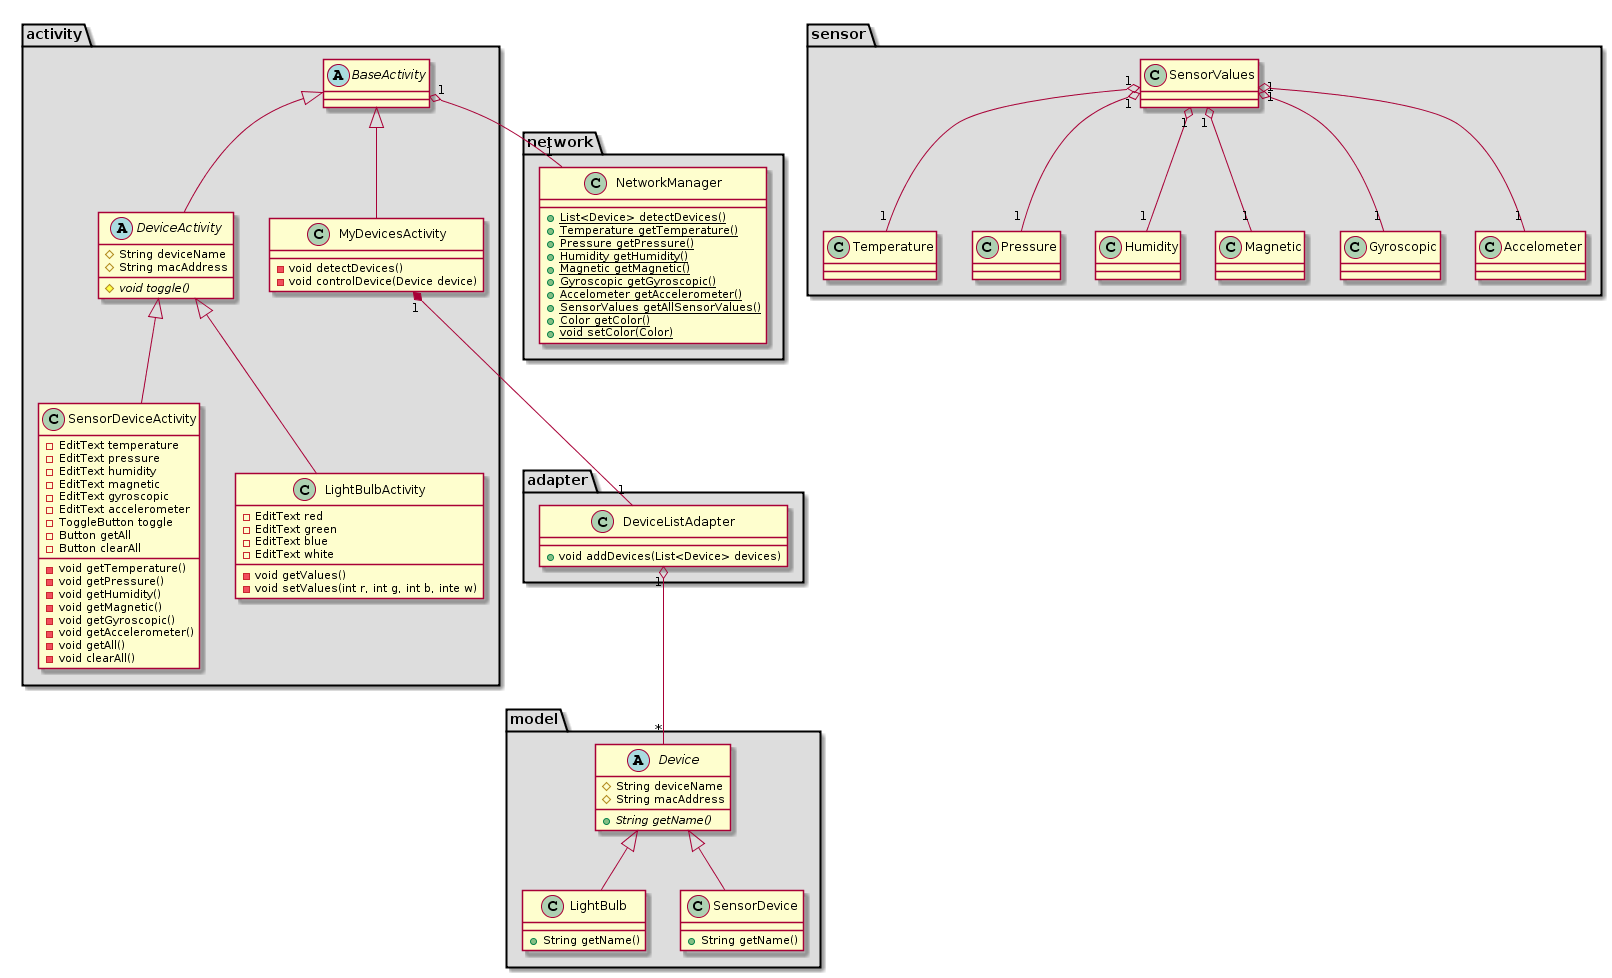
\includegraphics[width=1\textwidth]{class_diagram.png}
    \caption{The layout of the Light Bulb View}
    \label{fig:mylightbulbview}
\end{figure}
\begin{itemize}
\item{\textbf{BaseActivity:}} 
The BaseActivity for the application that will connect the Activities with the NetworkManager.
\item{\textbf{MyDeviceActivity:}} 
Is the start screen of the application. Will contain a ListView and has methods for detecting devices and control a device that was selected from the ListView.
\item{\textbf{DeviceListAdapter:}} 
Adapter that handles the list in MyDevicesActivity, the ListView can display any data provided that it is wrapped in a ListAdapter. 
\item{\textbf{Device:}} 
Is an Abstract class that controlls the two devices we are handling. 
\item{\textbf{SensorDevice:}} 
Class containing the SensorDevice information.
\item{\textbf{LightBulb:}}
Class containing the LightBulb information.
\item{\textbf{DeviceActivity:}} 
Is an abstract class that holds the shared parameters deviceName and macAddress. It also contains an abstract method toggle that controls the on/off switch on the devices.
\item{\textbf{SensorDeviceActivity:}} 
Is the controller in the interaction with the user in the SensorDevice View. Controls the TextView fields and the buttons that will retrieve information regarding the sensors from NetworkManager.
\item{\textbf{LightBulbActivity:}} 
Is the controller in the interaction with the user in the LightBulb View. Controls the EditText fields and the buttons that will retrieve and send information from/to the NetworkManager.
 
\item{\textbf{NetworkManager:}} 
Handles all the communication with the API. The different methods for controlling both receiving and setting data.
\item{\textbf{SensorValues:}} 
A superclass for the information of the different sensors.

\end{itemize}

\subsection{Rubrik för sekvensdiagram}
In progress..
\subsection{Packages}
\begin{itemize}
\item Network
\item Activity
\item Adapter
\item Model
\item Sensor
\end{itemize}

\end{document}